% ============================================================================
% October 17, 2026 rewrite of the empirical section. Sources, read Oct 17:
%   AHS: code/data/ahs_supply_snapshot/output_ahs_family_unit_menu_national/
%        ahs_stock_by_bedroom_tenure.csv, ahs_stock_by_room_tenure.csv,
%        ahs_children_space_mismatch.csv
%   PSID rooms, A2h: code/data/psid_followup_mar2026/output/
%        sa_rooms_first_birth_v2/A2h/coefficients.csv (full support, 1.47)
%        output/model/first_birth_rooms_event_20261010/measurement_bridge/
%        original/rooms_coefficients.csv (common support, 1.44)
%   PSID ownership and moves, A2h: code/data/psid_followup_mar2026/output/
%        sa_first_birth_outcomes_v3/summary.csv and window_path.csv
%   ACS (large homes, 12.8 pp gap): numbers carried over from the Oct 9 mock,
%        not re-read on Oct 17.
% ============================================================================

\section{Empirical Evidence}
\label{sec:empirical-evidence}

In this Section, I show some motivating evidence on housing changes around
the first birth using the Panel Study of Income Dynamics (PSID). I begin by
describing changes in housing at parenthood. Three to four years after the
birth, parents live in 1.4 more rooms than two to three years before it, a
31\% increase, and are 27 percentage points more likely to own their
home, up from 43\%. Both margins, space and ownership, are central to
the model of Section~\ref{sec:model}, and they crucially inform the
quantification in Section~\ref{sec:quant}. I then document the increased
salience of space among the reasons households give for moving. One to two
years after the birth, the probability of moving for more space rises by 2.1
percentage points, a 33\% increase over 6.4\%, while moves for
neighborhood reasons do not rise. Among households that move, the share
citing more space rises from 12\% to 27\% three to four years after the
birth.

\subsection{Data and Design}
\label{sec:emp-data-design}

The PSID has followed a representative sample of U.S. families and
their descendants since 1968, every year until 1997 and every two years
since. I use the waves from 1968 to 2023.

In this Section, I focus on four housing outcomes. ``Rooms'' is the number
of rooms in the home. ``Owner'' equals one if the household owns its home.
Households that moved since the previous interview are asked why they moved,
and I use the first reason they give. ``Moved for space'' equals one if the
household moved and its first reason is expansion of housing, such as more
space, and zero otherwise. ``Moved for neighborhood'' is defined in the same
way for neighborhood reasons, such as a better neighborhood or being closer to friends or
relatives; this category also includes moves to attend school.
Appendix~\ref{app:empirical-data} details the variables and the sample
construction.

I measure how housing changes around the first birth, relative to two to
three years before it and relative to adults who never have a child. I use
this reference, rather than the year before the birth, because households
may move ahead of a planned birth. Formally, let $Y_{it}$ be an outcome of
adult $i$ in survey year $t$ and $E_i$ the year of the first birth. I
estimate
\begin{equation}
Y_{it}=\alpha_i+\lambda_t+x_{it}'\gamma+\sum_{g}\sum_{k\neq -3/-2}\delta_{g,k}\,\mathbf 1\{E_i=g\}\,\mathbf 1\{t-E_i\in k\}+\varepsilon_{it},
\label{eq:event-study}
\end{equation}
where $\alpha_i$ and $\lambda_t$ are person and survey-year fixed effects,
$x_{it}$ contains indicators for age and education, $g$ indexes first-birth
years, and $k$ indexes two-year windows of event time $t-E_i$. The
coefficient $\delta_{g,k}$ is the change in $Y$ in window $k$ for adults
whose first birth is in year $g$, relative to the omitted window.

The treated group consists of adults who have a first child and who, two to
three years before the birth, were already the reference person or the
spouse of a household, so that their housing in the omitted window is that
of their own household.\footnote{The results are qualitatively similar when the sample includes,
at each interview, every woman who is the reference person or the spouse
of a household. For more detail, see
Appendix~\ref{app:empirical-two-samples}.} The control group consists of all adults who
never have a child; they carry no event-time indicators. To account for
effects that differ across cohorts of first births, I estimate
equation~\eqref{eq:event-study} with the estimator of
\citet{sunAbrahamDynamicEffects2021}.\footnote{Two-way fixed effects regressions with pooled event-time indicators are
biased when the effect of the birth differs across cohorts
\citep{goodmanbaconDifferenceinDifferencesVariationTreatment2021}. The
method of \citet{sunAbrahamDynamicEffects2021}, followed here, estimates a
separate path for each cohort of parents, compares it only with
never-parents, and averages the paths with the cohort shares.} I report
\begin{equation}
\hat\beta_k=\sum_g w_{g,k}\,\hat\delta_{g,k},
\label{eq:event-study-weights}
\end{equation}
where $w_{g,k}$ is the share of first-time parents observed in window $k$
whose first birth is in year $g$. I refer to $\beta_k$ as the housing response to the first birth in window $k$.
For example, $\beta_{+3/+4}$ is the change in $Y$ three to four years after
the first birth, relative to two to three years before it and relative to
the change among never-parents. Observations are weighted by the PSID longitudinal weight.

\subsection{Housing Around the First Birth}
\label{sec:emp-first-birth}

Figure~\ref{fig:emp-rooms-own} shows the response of housing choices around
the first birth. Panel (a) shows the path of housing size. Two to three years before the birth, parents live in 4.71 rooms.
Rooms rise by 0.62 in the birth window (+13\%) and by 1.44 three to
four years after the birth (+31\%), and rise more slowly afterwards, to 1.8 more rooms eleven or more years after the birth. In the windows before the reference, the coefficients are below a tenth of a room.
The adjustment is large and concentrated around the birth: two-thirds of
the long-run increase occurs by one to two years after it. This indicates
that, although the analysis does not rule out anticipation, children
acquire particular salience around the birth itself, and the demand for
space rises abruptly.

\begin{figure}[t]
\centering
\caption{Rooms and Ownership Around the First Birth (PSID)}
\label{fig:emp-rooms-own}
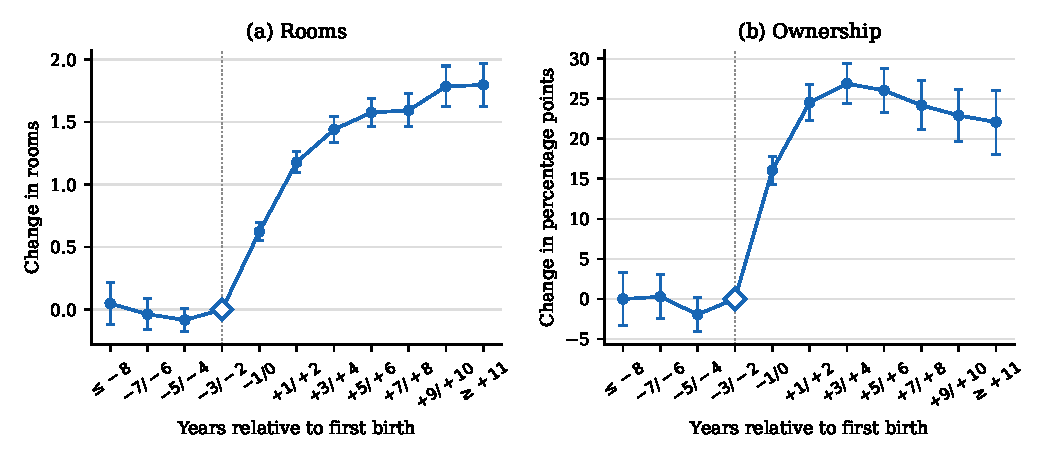
\includegraphics[width=\linewidth]{figures/first_birth_rooms_ownership_2x1.pdf}
\par\medskip
\begin{minipage}{0.92\linewidth}
\footnotesize Note: This figure shows the estimates of $\beta_k$ in
equation~\eqref{eq:event-study-weights}, in two-year windows, with 95\% confidence intervals. Rooms use the sample on which the model's
event study is measured ($N = 112{,}148$); ownership uses its available observations
($N = 111{,}272$). The hollow marker is the omitted reference window.
\end{minipage}
\end{figure}

Panel (b) shows the path of homeownership. Two to three years before the birth, 43\% of parents own
their home. Ownership rises by 16 percentage points in the birth window
(+37\%) and by 27 points three to four years after the birth (+63\%).\footnote{Appendix~\ref{app:empirical-two-samples} also shows the probability
of moving since the previous interview. It is highest two to three years
before the birth, at 54\%, and is 17 percentage points lower one to two years
after the birth and 21 points lower three to four years after it
(Table~\ref{tab:app-tenure-moves}). \citet{couillardBuildBabyBuild2025} finds
the same anticipation of births in the ACS.}

Figure~\ref{fig:emp-move-reasons} explores the reasons households give for
moving. Panel (a) shows the probability of moving for more space, and panel
(b) the probability of moving for neighborhood reasons. Two to three years before the birth, 6.4\% of households
move for more space and 3.0\% for neighborhood reasons. One to two years
after the birth, the probability of moving for more space is 2.1 percentage
points higher (+33\%), while the probability of moving for neighborhood
reasons does not rise.\footnote{Among households that move, the share citing
more space rises from 12\% to 27\% three to four years after the birth
(Table~\ref{tab:app-tenure-moves}). A larger home could also come from a
move to a cheaper location rather than from a larger outlay on housing.
Among households that already owned two to three years before the birth,
house value rises by 30\% three to four years after the birth and value per
room by 11\%, and moves across state lines become less frequent
(Appendix~\ref{app:house-value}).} This highlights a strong role for concerns about size of the dwelling at childbirth.

\begin{figure}[t]
\centering
\caption{Reasons for Moving Around the First Birth (PSID)}
\label{fig:emp-move-reasons}
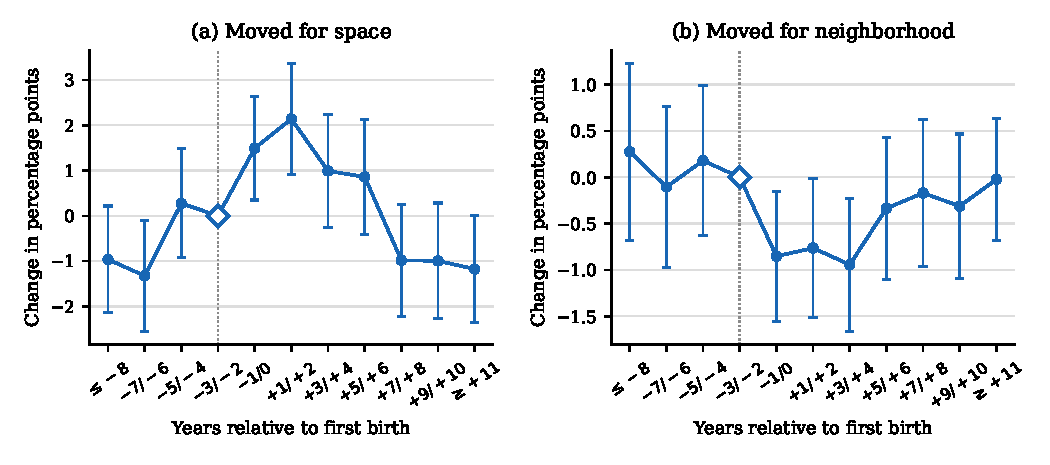
\includegraphics[width=\linewidth]{figures/first_birth_move_reasons_2x1.pdf}
\par\medskip
\begin{minipage}{0.92\linewidth}
\footnotesize Note: This figure shows the estimates of $\beta_k$ in
equation~\eqref{eq:event-study-weights}, in percentage points, with 95\% confidence intervals ($N = 116{,}697$). The outcomes are
probabilities among all households, including those that did not move. The
hollow marker is the omitted reference window.
\end{minipage}
\end{figure}

In summary, housing is particularly relevant around childbirth, which increases the desire for size and leads people to ownership. The complex web of interactions that take place in the data motivates the writing of a model. Agents need to make a set of intertwined decisions. Having children increases desire for space, and it is easier to get this space by owning (see Appendix~\ref{app:housing-stock}). Owning requires saving to be able to afford a down payment, and children also increase general expenses. The model developed in Section~\ref{sec:model} tries to model the interaction between these forces, in order to discipline their relative strength and potential for policy. The evidence detailed above not only motivates, but also informs my modeling choices. Because the demand
for space rises at the first birth, fertility and housing are chosen
jointly: a family needs a minimum amount of space before additional rooms
raise its utility. In the U.S. housing stock, large homes are mostly owned
rather than rented
(Appendix~\ref{app:housing-stock}). The model captures this by
capping the size of rental units, so that a family that wants a large home
must buy it and make a down payment; the wealth of young households then
matters for when they have children, and childbirth affects the desire to own, as in the data.
